% =====================================================================
%  Fixed-bond MD does not rank ADC linkers
%  Modern two-column coloured preprint template (chemRxiv-ready).
%  Compile:  latexmk -pdf -bibtex manuscript.tex
%  (TeX Live installed locally; figures = vector PDFs in ../figures/.)
% =====================================================================
\documentclass[10pt,twocolumn]{article}

\usepackage[letterpaper,margin=1.7cm,columnsep=0.7cm]{geometry}
\usepackage[T1]{fontenc}
\usepackage[utf8]{inputenc}
\usepackage{lmodern}
\usepackage{microtype}
\usepackage{amsmath,amssymb}
\usepackage[version=4]{mhchem}
\usepackage{graphicx}
\graphicspath{{../figures/}}
\usepackage{xcolor}
\usepackage{colortbl}
\usepackage{booktabs}
\usepackage{array}
\usepackage{enumitem}
\usepackage{titlesec}
\usepackage{caption}
\usepackage{tcolorbox}
\usepackage{fancyhdr}
\usepackage[numbers,sort&compress]{natbib}
\usepackage[hidelinks]{hyperref}

% ---- palette -------------------------------------------------------
\definecolor{ink}{HTML}{17314A}      % dark navy (title / headings)
\definecolor{accent}{HTML}{0072B2}   % primary blue
\definecolor{accent2}{HTML}{C2570C}  % burnt orange
\definecolor{tint}{HTML}{EAF3FA}     % light blue fill
\definecolor{tint2}{HTML}{FBEDE2}    % light orange fill
\definecolor{rule}{HTML}{9DC3E0}

\hypersetup{colorlinks=true,linkcolor=accent2,citecolor=accent,urlcolor=accent}

% ---- headings ------------------------------------------------------
\titleformat{\section}{\sffamily\large\bfseries\color{ink}}{\thesection}{0.55em}{}[{\color{rule}\titlerule[1pt]}]
\titleformat{\subsection}{\sffamily\normalsize\bfseries\color{accent}}{\thesubsection}{0.5em}{}
\titlespacing*{\section}{0pt}{1.4ex}{0.7ex}
\titlespacing*{\subsection}{0pt}{1.1ex}{0.4ex}
\titleformat{\paragraph}[runin]{\sffamily\bfseries\color{ink}}{}{0pt}{}[.\hspace{0.4em}]

% ---- captions ------------------------------------------------------
\captionsetup{font=small,labelfont={bf,sf,color=accent},labelsep=period,skip=4pt}

% ---- running head --------------------------------------------------
\pagestyle{fancy}\fancyhf{}
\fancyhead[L]{\footnotesize\sffamily\color{ink}Evaluating generative ADC linkers}
\fancyhead[R]{\footnotesize\sffamily\color{ink}\thepage}
\renewcommand{\headrulewidth}{0pt}
\fancypagestyle{plain}{\fancyhf{}\renewcommand{\headrulewidth}{0pt}}

% ---- coloured callout box ------------------------------------------
\newtcolorbox{keybox}{colback=tint,colframe=accent,boxrule=0.7pt,
  left=6pt,right=6pt,top=4pt,bottom=4pt,arc=2pt,
  fonttitle=\sffamily\bfseries\color{ink}}

% ---- full-width title + abstract (spans both columns) --------------
\title{Evaluating generative antibody--drug conjugate linkers: chemical validity, covalent dynamics, and an FDA-anchored control}
\author{}\date{}

\makeatletter
\renewcommand{\@maketitle}{%
  \vspace*{-1.0em}
  {\sffamily\bfseries\LARGE\color{ink}\@title\par}
  \vspace{0.7em}
  {\large\color{ink}Ga\"el Coulombe\textsuperscript{1} \quad Hazem Mslati\textsuperscript{2}\par}
  \vspace{0.2em}
  {\small\textsuperscript{1}Universit\'e de Sherbrooke, Sherbrooke, QC, Canada \;\textbullet\; \textsuperscript{2}Affiliation TBD\par}
  \vspace{0.1em}
  {\small Corresponding author: \href{mailto:gael.coulombe@usherbrooke.ca}{gael.coulombe@usherbrooke.ca}\par}
  \vspace{0.5em}
  {\color{accent}\rule{\textwidth}{1.2pt}}\par
  \vspace{0.7em}
  \noindent\colorbox{tint}{\parbox{\dimexpr\textwidth-2\fboxsep-2\fboxrule}{%
    \small\setlength{\parindent}{0pt}%
    {\sffamily\bfseries\color{accent}ABSTRACT.\hspace{0.4em}}%
    Generative 3D models can now propose antibody--drug conjugate (ADC) linkers, shifting the open
    problem from \emph{generation} to \emph{evaluation}. We fine-tune DiffLinker on 73 ADC
    linker--payloads and show it learns ADC linker chemistry without memorization: cleavable motifs
    (Val-Cit, urea, Gly-Gly-Phe-Gly) emerge at 10--81\,\% versus 0--4\,\% in the zero-shot baseline,
    with median Tanimoto similarity 0.44--0.59 to the training set and zero near-copies across 1000
    generations. The dominant practical failure is not the model but \textbf{chemical validity}:
    outputs routinely lose connectivity, valence, and stereochemistry, leaving only ${\approx}10$ fully
    3D-valid candidates per 100 (Wilson 95\,\% CI 7.8--13.2) after a fail-closed validity gate. We then
    ask whether classical covalent molecular dynamics (MD) can \emph{rank} the survivors. Building
    covalent trastuzumab-Fab/HER2 complexes at Cys214 and running 50\,ns each, all candidates are
    \textbf{grossly stable} (covalent bond 1.81\,\AA, secondary structure preserved, per-domain
    C$\alpha$ RMSD 1.2--1.8\,\AA). An apparent payload-stability ranking is traced to a
    \textbf{topology artifact} --- a pentavalent conjugation carbon --- that vanishes and partially
    inverts once corrected. A pre-registered $N{=}3$ replicate study finds no separation (Welch
    $p{=}0.157$). Grafting the FDA-approved brentuximab-vedotin linker onto the identical scaffold
    yields a payload metric statistically indistinguishable from the generated candidates
    ($p{=}0.41$, $0.20$). Fixed-bond MD payload RMSD is non-discriminative for ADC linkers because the
    chemistry that would discriminate them --- succinimide hydrolysis, retro-Michael deconjugation,
    local $pK_\mathrm{a}$ --- is absent from the model by construction.\par}}%
  \vspace{1.1em}
}
\makeatother

% =====================================================================
\begin{document}
\maketitle
\thispagestyle{fancy}

% =====================================================================
\section{Introduction}

Antibody--drug conjugates (ADCs) couple the specificity of a monoclonal antibody to a cytotoxic payload
through a chemical linker.\cite{drago2021} The linker is not a passive tether: its stability in
circulation governs premature payload release, off-target toxicity, and ultimately the therapeutic
index.\cite{shen2012} Designing a linker is therefore a multi-objective problem in which the hard
constraint --- plasma stability of the conjugation site --- is precisely the property that is hardest to
compute.

Recent work applies 3D generative diffusion models to \emph{linker} design, holding the payload fixed and
generating the spacer that connects it to the antibody-side conjugation handle.\cite{igashov2024} These
methods are improving quickly. What is rarely stress-tested is the \emph{evaluation} step that follows
generation --- the procedure that is supposed to tell us which generated linker is best. In most pipelines
it is assumed reliable: a potency surrogate, or a short molecular-dynamics (MD) simulation read out
through a stability proxy such as payload root-mean-square deviation (RMSD).

This paper stress-tests that assumption, and it fails --- cleanly, reproducibly, and against a clinical
control. We report a complete generate\,$\rightarrow$\,gate\,$\rightarrow$\,build\,$\rightarrow$\,simulate\,$\rightarrow$\,evaluate
pipeline (Figure~\ref{fig:pipeline}) and show that while DiffLinker generates chemically plausible, novel
ADC linkers, \textbf{neither a 2D potency classifier nor fixed-bond covalent MD can reliably rank them}.
The strongest evidence is a positive control: replacing a generated linker with the authentic,
FDA-approved brentuximab-vedotin linker and rerunning the identical simulation leaves the clinical linker
statistically indistinguishable from our generated candidates.

\begin{figure}[t]
\centering
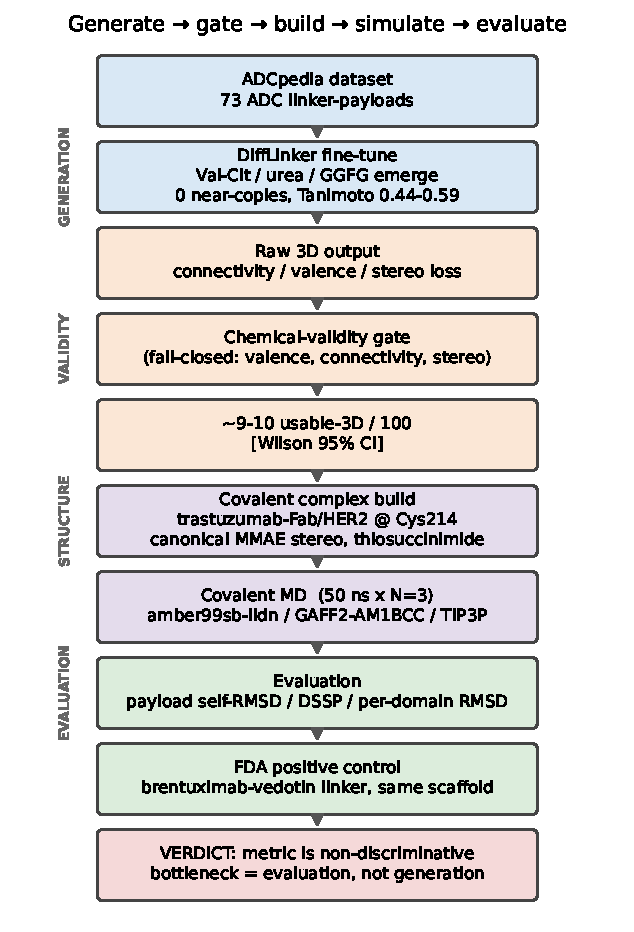
\includegraphics[width=0.82\linewidth]{fig1_pipeline}
\caption{The generate\,$\rightarrow$\,chemical-validity gate\,$\rightarrow$\,covalent build\,$\rightarrow$\,covalent
MD\,$\rightarrow$\,evaluation pipeline, with the FDA positive control.}
\label{fig:pipeline}
\end{figure}

\noindent\textbf{Contributions.}
\begin{itemize}[leftmargin=1.1em,itemsep=1pt,topsep=2pt]
\item A reproducible DiffLinker\,$\rightarrow$\,validity-gate\,$\rightarrow$\,covalent-MD pipeline for ADC
linkers at a cysteine thiosuccinimide site (Figure~\ref{fig:pipeline}).
\item Evidence that \textbf{chemical validity --- not generation --- is the dominant practical
bottleneck}, with a fail-closed valence/connectivity/stereo gate as the operative screen
(Figure~\ref{fig:funnel}).
\item A documented \textbf{ranking artifact}: a covalent-topology valence error produced a confident but
spurious payload ranking that disappears under correction (Figure~\ref{fig:artifact}).
\item A \textbf{pre-registered $N{=}3$ test plus an FDA positive control} showing fixed-bond MD payload
RMSD does not discriminate generated linkers from one another or from an approved clinical linker
(Figures~\ref{fig:n3}--\ref{fig:vedotin}).
\item A cross-cutting lesson: \textbf{surface metrics (bond length, classifier AUC, score) mask
structural errors; adversarial validation is required} (Table~\ref{tab:findings}).
\end{itemize}

\section{Background}

\paragraph{3D diffusion for linker generation}
DiffLinker\cite{igashov2024} is an $E(n)$-equivariant diffusion model pretrained on
GEOM-Drugs\cite{axelrod2022} that generates a linker between fixed fragments. Its native output is
atomistic --- predicted 3D coordinates and atom types --- without bond orders, perceived afterward from
interatomic distances. This format is the origin of the chemical-validity problem of
Section~\ref{sec:validity}.

\paragraph{What sets ADC linker stability}
The cysteine--maleimide adduct anchoring many clinical ADCs is metastable: the thiosuccinimide can
undergo retro-Michael elimination and thiol exchange with plasma thiols (albumin, glutathione), releasing
payload prematurely.\cite{shen2012} The competing, stabilizing pathway --- hydrolytic ring-opening of the
succinimide, catalysed by a proximal basic residue --- renders the adduct resistant to
retro-Michael.\cite{lyon2014} Stability is thus controlled by bond-breaking chemistry, local
$pK_\mathrm{a}$, and the conjugation-site electrostatic microenvironment, none of which is represented in
a classical fixed-bond force field.

\paragraph{Existing ADC scoring}
Potency classifiers such as AMM predict cytotoxicity from a 2D conjugate representation plus biological
context.\cite{mslati2026} MD-derived geometric proxies are sometimes used as stability surrogates. Both
assume the discriminating signal is captured; we test that directly.

\section{Methods}

\subsection{Generation}
DiffLinker was fine-tuned on 73 unique ADC linker--payloads spanning three conjugation chemistries
(cysteine, lysine, click), recovered from the ADCpedia dataset\cite{mslati2026} by a payload-anchored
decomposition (coverage 98\,\%). Two fine-tunes are reported (Table~\ref{tab:motifs}): a cysteine-only
set (43 unique L/Ps) and the full multi-site superset (73 L/Ps, the figure quoted above). The candidates
carried forward to covalent MD were generated from the best-yield cysteine-line checkpoint at the
operational linker size; full dataset, sweep, and checkpoint details are in the SI. The numerically
stabilized recipe (isfinite loss guard, restored
pretraining optimizer state, learning rate $1\times10^{-5}$, batch 4, early stopping on denoising
validation loss) is in the SI. Full generation methodology is supporting material --- prior to this
paper's contribution.

\subsection{Chemical-validity gate}
A two-level gate. \textbf{Level A} (ligand, RDKit\cite{rdkit}): sanitizable; single connected component;
no undefined stereocenters; correct maleimide/thiosuccinimide oxidation state. \textbf{Level B}
(conjugate topology): per-atom bond count vs.\ element valence maximum, fail-closed at build time --- the
guard that auto-catches the over-valent conjugation carbon of Section~\ref{sec:artifact}.

\subsection{Covalent complex construction}
Receptor 1N8Z (trastuzumab Fab + HER2 ectodomain)\cite{cho2003}, cleaned with PDBFixer (pH 7.4). The
conjugation cysteine was chosen by side-chain SASA: \textbf{A:Cys214} (SG-SASA 43.75\,\AA$^2$, the most
exposed free cysteine). Because DiffLinker outputs lose stereochemistry through the
coordinate\,$\rightarrow$\,SDF step, canonical MMAE stereochemistry (10 stereocenters) was reimposed by
CIP-driven iterative chiral-tag assignment (10/10 verified from 3D coordinates). Conjugation used a
maleimide Michael addition; the ligand was aligned so the thioether carbon superimposed on the Cys214 SG
(C--SG $=1.80$\,\AA), with rotational clash minimization.

\subsection{MD protocol}
GROMACS 2025\cite{abraham2015}; amber99sb-ildn\cite{lindorfflarsen2010} protein, GAFF2\cite{wang2004}
with AM1-BCC charges\cite{jakalian2002} (acpype\cite{sousadasilva2012}) ligand, TIP3P
water\cite{jorgensen1983}, 0.15\,M NaCl, dodecahedral box (1.2\,nm). The covalent C--SG linkage was a
\textbf{true bond} (ligand merged into the light-chain moleculetype so 1-2/1-3 exclusions generate
correctly), held by a harmonic term --- a fixed-bond covalent model. Protocol: minimization
$\rightarrow$ 100\,ps NVT $\rightarrow$ 100\,ps NPT (restrained) $\rightarrow$ 50\,ns production at 2\,fs.
A fail-closed gate preceded every run: grompp clean, conjugation sulfur exactly two bonds (C$\beta$ +
ligand carbon, no retained thiol proton), thioether sulfur type, conserved chain charge.

\subsection{Evaluation metrics}
Analyses used PBC-corrected trajectories (\texttt{-pbc whole}$\rightarrow$\texttt{nojump}). We separate
\emph{integrity checks} (C--SG distance, ligand--protein minimum distance --- bonded-topology-enforced,
$\sigma{\approx}0.04$\,\AA) from \emph{behavioral observables}. Per-domain C$\alpha$ RMSD was
self-fitted per domain --- correct for a multi-domain Fab--HER2 assembly whose whole-complex RMSD is
dominated by rigid-body motion. Secondary structure was tracked by DSSP.\cite{kabsch1983} Payload
behavior used the \textbf{MMAE-core (51 heavy atoms) self-fitted RMSD}, isolating internal deformation
from whole-ligand swing; the core was extracted by an order-verified substructure match that excludes the
PABC carbamate carbon (which otherwise aliases the match).

\subsection{Positive control}
The authentic mc-Val-Cit-PAB-MMAE linker--payload of brentuximab vedotin (CAS 646502-53-6,
\ce{C68H105N11O15}, MW 1316.65) was conjugated to the \textbf{same} Cys214 on the \textbf{same} scaffold
with the \textbf{same} thiosuccinimide chemistry, force field, and $50\,\text{ns}\times3$ protocol ---
everything constant except the linker.

\subsection{Statistical design (pre-registered)}
$N{=}3$ independent replicates per system (rep~1 continued from NPT velocities; reps~2--3 fresh velocity
draws, distinct seeds, \texttt{continuation\,=\,no}). Metric: MMAE-core self-RMSD over 25--50\,ns.
Pre-registered separation criterion: mean\,$\pm$\,SD ranges disjoint \textbf{and} Welch $p<0.05$.

% =====================================================================
\section{Results}

\subsection{DiffLinker learns ADC chemistry without memorizing}
After fine-tuning, the model produces cleavable-linker signatures absent from the pretrained baseline:
Val-Cit ureido, urea, and Gly-Gly-Phe-Gly motifs emerge at 10--81\,\% versus 0--4\,\% zero-shot at
matched size (Table~\ref{tab:motifs}). This is learning, not copying: across 1000 generations there were
\textbf{zero near-copies} (Tanimoto $>0.85$), and median Tanimoto to the training set was 0.44--0.59. The
fine-tune also unlocked generation at ADC linker length, which the zero-shot model could not reach. (Two
intrinsic tradeoffs --- chemistry vs.\ connectivity along size, and target-specificity vs.\ topological
diversity along the training distribution --- are characterized in the SI; they do not affect the
conclusions here.)

\begin{table}[t]
\caption{ADC-motif emergence and novelty, fine-tuned vs.\ zero-shot (matched size). Zero near-copies
(Tanimoto $>0.85$) per 1000 generations across all fine-tuned configurations.}
\label{tab:motifs}
\centering\small
\setlength{\tabcolsep}{5pt}
\begin{tabular}{@{}llrrr@{}}
\toprule
\rowcolor{tint}\sffamily Model & \sffamily size & \sffamily Val-Cit & \sffamily Urea & \sffamily med.\ Tan. \\
\midrule
Zero-shot          & 20 & 0\,\%  & 0\,\%  & 0.30 \\
Fine-tuned (cys)   & 20 & 23\,\% & 35\,\% & 0.58 \\
Fine-tuned (cys)   & 60 & 64\,\% & 81\,\% & 0.44 \\
Fine-tuned (multi) & 20 & 10\,\% & 13\,\% & 0.59 \\
Fine-tuned (multi) & 60 & 43\,\% & 69\,\% & 0.46 \\
\bottomrule
\end{tabular}
\end{table}

\subsection{Chemical validity, not generation, is the bottleneck}
\label{sec:validity}
DiffLinker's atomistic output systematically fails three chemical-validity criteria.
\emph{Connectivity}: only ${\approx}30$--45\,\% of outputs are a single connected fragment at the
operational size. \emph{Valence}: bond perception leaves under- or over-coordinated atoms.
\emph{Stereochemistry}: the coordinate\,$\rightarrow$\,SDF conversion strips stereochemistry
irrecoverably, so the active configuration of the payload (e.g.\ MMAE's 10 stereocenters) must be
reimposed explicitly. After the fail-closed gate, only \textbf{${\approx}10$ fully 3D-valid candidates
survive per 100 generated} (Wilson 95\,\% CI 7.8--13.2; Figure~\ref{fig:funnel}). An industrial campaign
must therefore oversample by an order of magnitude, and the validity gate --- not the generator --- is
the operative screen: a millisecond-cost gate does work the MD cannot.

\begin{figure}[t]
\centering
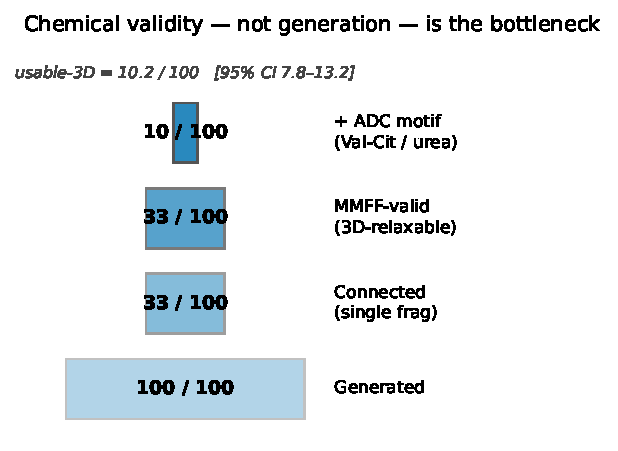
\includegraphics[width=\linewidth]{fig2_yield_funnel}
\caption{Usable-3D yield funnel. After the fail-closed gate, ${\approx}10$ of every 100 generated
molecules are connected, valence-correct, stereo-correct, and ADC-motif-bearing.}
\label{fig:funnel}
\end{figure}

\subsection{Gross MD stability: all candidates pass}
All four lead candidates are stable over 50\,ns at the coarse level (Figure~\ref{fig:gross},
Table~\ref{tab:gross}). The covalent thioether holds at a mean C--SG of 1.81\,\AA{} (no drift) in every
run. Per-domain C$\alpha$ RMSD shows the Fab is internally rigid (light/heavy chain 1.2--1.6\,\AA), with
elevated values confined to the intrinsically flexible HER2 peripheral domains I and IV
(Figure~\ref{fig:gross}a). Secondary structure is preserved: DSSP-structured fraction stays at
${\approx}43$\,\% (SD $<1.1$\,\%; Figure~\ref{fig:gross}b), the decisive test against unfolding. The
payload stays attached and in contact; no dissociation occurs. Candidates~1 and~8
(Table~\ref{tab:gross}) retain the first-pass junction topology later corrected in
Section~\ref{sec:artifact}; this does not affect their gross-stability classification, because the
C--SG distance (a harmonic term), the per-domain C$\alpha$ RMSD, and DSSP are all determined away from
the ligand junction and are invariant to its valence --- the defect perturbs only the payload's internal
self-RMSD. The discrimination analysis (Section~\ref{sec:artifact} onward) is therefore restricted to the
valence-corrected candidates~4 and~5 plus the control. At the coarse level the model behaves correctly
--- which sets up the discrimination question: can it tell the candidates apart?

\begin{figure*}[t]
\centering
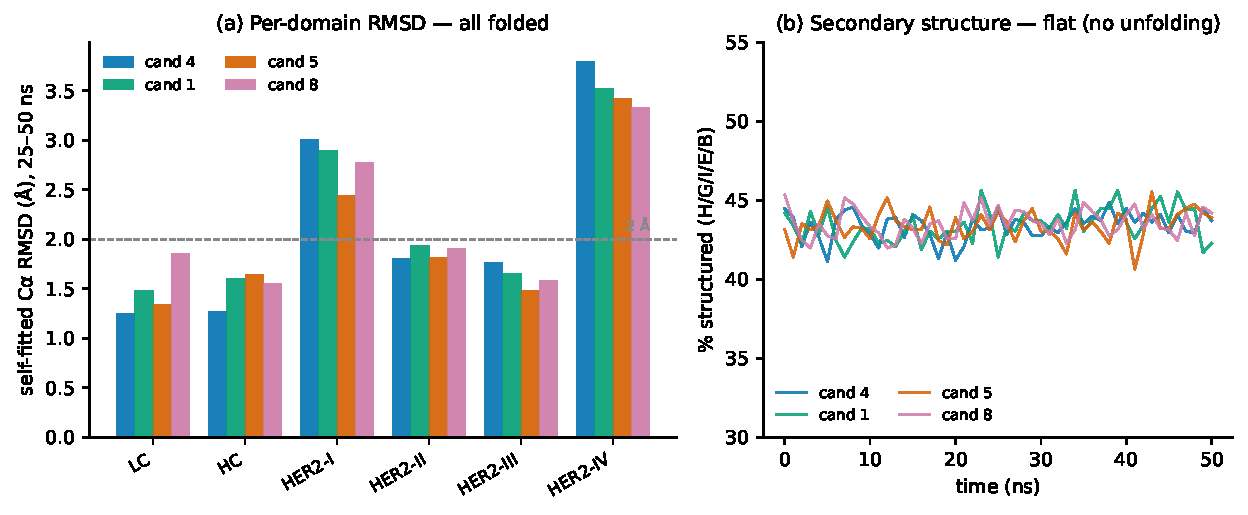
\includegraphics[width=0.9\linewidth]{fig3_gross_stability}
\caption{Gross MD stability (50\,ns). (a)~Per-domain self-fitted C$\alpha$ RMSD: the Fab is internally
rigid; elevated RMSD is confined to HER2 peripheral domains I and IV. (b)~DSSP structured fraction is
flat (${\approx}43$\,\%, SD $<1.1$\,\%) for all four candidates --- no unfolding.}
\label{fig:gross}
\end{figure*}

\begin{table}[t]
\caption{Gross MD stability, per candidate (means over 25--50\,ns, computed from the trajectories). LC/HC
= light/heavy chain; HER2 = whole ectodomain. All verdicts: \textbf{stable}.}
\label{tab:gross}
\centering\small
\setlength{\tabcolsep}{4.5pt}
\begin{tabular}{@{}lccccc@{}}
\toprule
\rowcolor{tint}\sffamily Cand. & \sffamily C--SG & \sffamily DSSP & \sffamily LC/HC & \sffamily HER2 & \sffamily verdict \\
\rowcolor{tint}\sffamily (output) & \sffamily (\AA) & \sffamily (\%) & \sffamily (\AA) & \sffamily (\AA) & \\
\midrule
4 (486) & 1.81 & 43.4$\pm$0.9 & 1.2/1.3 & 3.8 & stable \\
1 (219) & 1.81 & 43.4$\pm$1.1 & 1.5/1.6 & 3.8 & stable \\
5 (345) & 1.81 & 43.4$\pm$0.9 & 1.3/1.6 & 2.9 & stable \\
8 (106) & 1.81 & 43.5$\pm$0.9 & 1.9/1.6 & 3.8 & stable \\
\bottomrule
\end{tabular}
\end{table}

\subsection{The ranking artifact}
\label{sec:artifact}
It initially appeared so. On the first-pass topologies, candidate~4 looked markedly more rigid than
candidate~5 (MMAE-core self-RMSD 1.21 vs.\ 4.26\,\AA; Figure~\ref{fig:artifact}, grey), with a more
compact payload and fewer contacts --- a clean apparent ranking. Adversarial inspection of the junction
revealed the cause: the thioether bond had been added to the ligand carbon \textbf{without removing one
hydrogen}, producing a \textbf{pentavalent carbon}. GROMACS does not check valence, so it ran; a
distance-only check passed because the harmonic bond holds its length regardless. The over-constrained
junction clamped the payload, manufacturing the apparent rigidity.

\begin{figure*}[t]
\centering
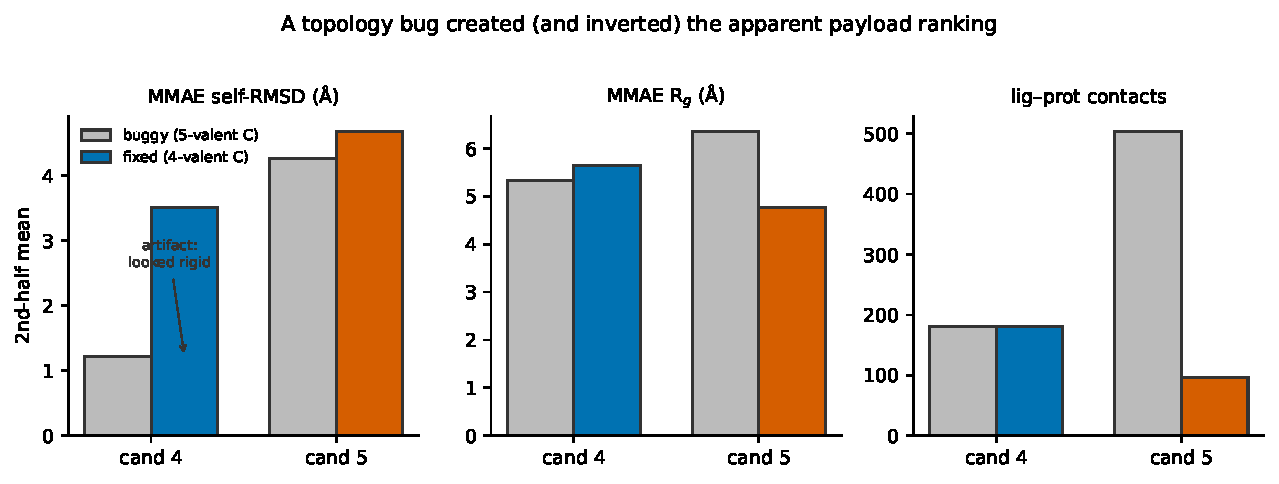
\includegraphics[width=0.92\linewidth]{fig4_artifact}
\caption{The ranking artifact. Buggy topology (pentavalent conjugation carbon, grey) vs.\ corrected
tetravalent thioether (colour). The apparent ``candidate~4 more rigid'' ranking disappears (self-RMSD)
and the secondary metrics ($R_g$, contacts) invert once the valence is corrected.}
\label{fig:artifact}
\end{figure*}

Correcting the valence (deleting one hydrogen, restoring a tetrahedral CH(S) thioether) erases the
ranking. Candidate~4's self-RMSD rises from 1.21 to 3.51\,\AA{} --- into candidate~5's range --- and the
secondary metrics invert: candidate~5, which had looked worst, becomes \emph{more} compact
($R_g$ $6.36\rightarrow4.77$\,\AA) and \emph{less} adsorbed (contacts $504\rightarrow96$) than
candidate~4 (Figure~\ref{fig:artifact}, colour). The apparent ``candidate~4 $>$ candidate~5'' ranking was
a chemistry-bug artifact, not a molecular property. (This was the second instance of the same failure
mode: an earlier defect left the cysteine thiol proton on the conjugated sulfur, also passing a
distance-only check --- Table~\ref{tab:findings}.)

\subsection{Replicates: no separation}
With correct chemistry, do the candidates separate beyond run-to-run noise? Three independent replicates
(Figure~\ref{fig:n3}) give candidate~4 $=3.15\pm0.96$\,\AA{} and candidate~5 $=4.33\pm0.30$\,\AA. The
means differ by 1.18\,\AA, but Welch gives $t=-2.04$, $\mathrm{df}=2.40$, $p=0.157$, with overlapping
ranges --- \textbf{no separation}. Candidate~4's intra-candidate spread (SD 0.96\,\AA, replicates
2.06--3.87\,\AA) is as large as the inter-candidate gap: the payload is not configurationally converged at
50\,ns, so a self-RMSD-vs-start ``ranking'' reads drift from an arbitrary pose. $N{=}3$ is low-powered
($\mathrm{df}{\approx}2.4$) and detects only a large effect --- it does not prove the candidates
identical; it proves no signal survives noise at this cost.

\begin{figure}[t]
\centering
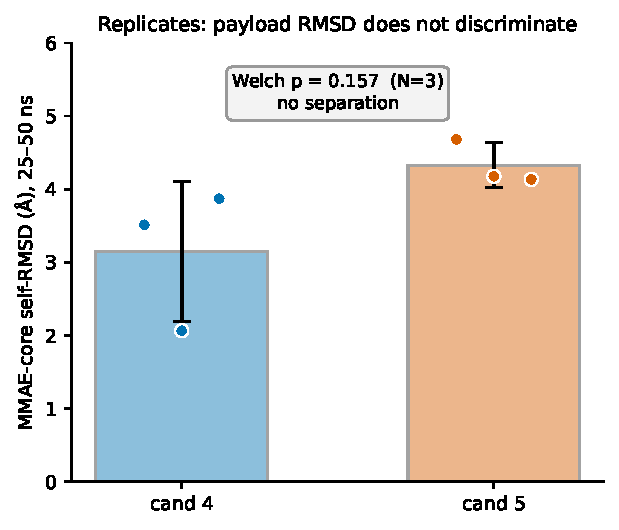
\includegraphics[width=0.86\linewidth]{fig5_n3_selfrmsd}
\caption{$N{=}3$ replicates, candidates 4 vs.\ 5. Points are replicates, bars mean\,$\pm$\,SD. No
separation (Welch $p=0.157$); intra-candidate spread $\approx$ inter-candidate gap.}
\label{fig:n3}
\end{figure}

\subsection{Positive control: an FDA linker is indistinguishable}
The decisive test removes the power objection. Grafting the FDA-approved brentuximab-vedotin linker onto
the identical scaffold and rerunning the identical $N{=}3$ protocol gives a payload self-RMSD of
$3.75\pm0.54$\,\AA{} --- landing \textbf{between} the two candidates, inside their envelope
(Figure~\ref{fig:vedotin}), non-significant against both (vedotin vs.\ candidate~4 $p=0.41$; vs.\
candidate~5 $p=0.20$).

\begin{figure}[t]
\centering
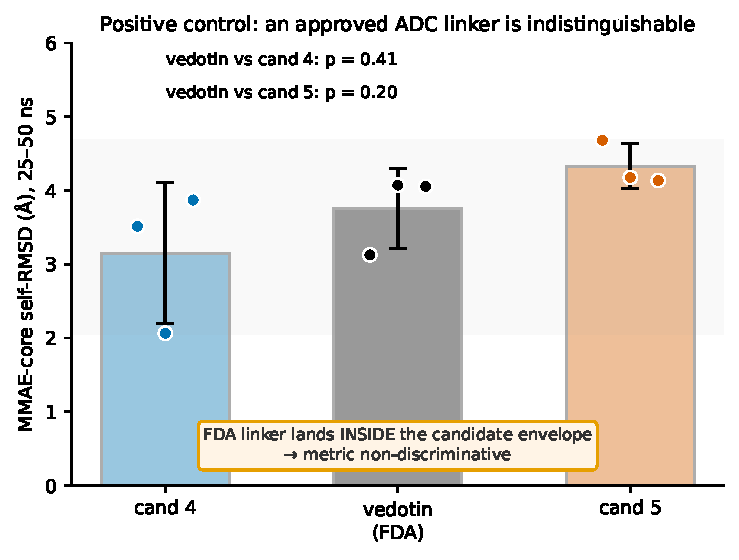
\includegraphics[width=0.95\linewidth]{fig6_vedotin_control}
\caption{Positive control. The FDA-approved brentuximab-vedotin linker (black), conjugated to the same
scaffold and run identically, gives a payload self-RMSD inside the generated-candidate envelope and
statistically indistinguishable from both ($p=0.41$, $0.20$).}
\label{fig:vedotin}
\end{figure}

\begin{keybox}
\textbf{Key result.} A metric that cannot distinguish a clinically approved ADC linker from arbitrary
generated candidates is non-discriminative \emph{by demonstration} --- independent of statistical power.
Encouragingly, the generated candidates occupy the same payload-dynamics regime as an approved ADC, so
they are physically realistic.
\end{keybox}

\subsection{Why the metric fails --- by construction}
The failure is structural, not a sampling deficiency to be cured with more nanoseconds. The model has a
fixed harmonic covalent bond, no bond-breaking, no constant-pH, and no plasma thiols --- it omits exactly
the chemistry that sets ADC stability: succinimide ring-opening, retro-Michael, local $pK_\mathrm{a}$.
Consistent with this, static + dynamic analysis of the Cys214 site (Figure~\ref{fig:site}) finds it
acidic near the sulfur ($pK_\mathrm{a}{\approx}9.9$; nearest base Arg211 at 8.9\,\AA, beyond catalytic
range), with only transient, flexible-linker-driven basic contacts --- weak self-stabilization. But the
site is \textbf{shared across all candidates}, so it annotates the site, not the linker. \emph{The
quantity that would rank candidates is precisely the quantity the cheap model omits.}

\begin{figure}[t]
\centering
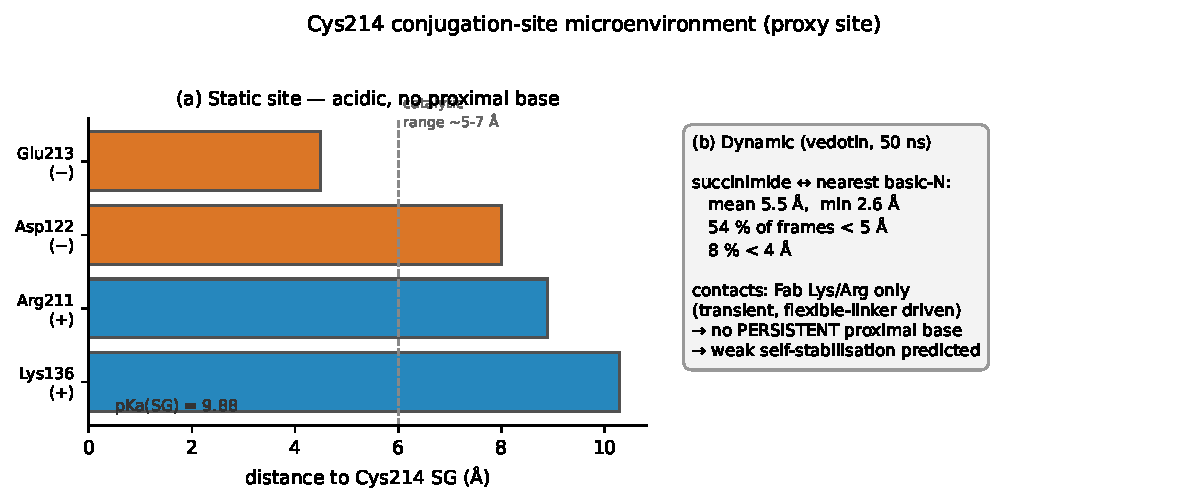
\includegraphics[width=\linewidth]{fig7_site_microenv}
\caption{Cys214 microenvironment. (a)~Static: the immediate SG environment is acidic; the nearest basic
residue is beyond catalytic range. (b)~Dynamic (vedotin, 50\,ns): only transient basic contacts. Weak
self-stabilization --- and, being shared across candidates, the site cannot rank linkers.}
\label{fig:site}
\end{figure}

The 2D potency classifier (AMM) fails to rank for a parallel reason: its label is saturated. A potent
payload (MMAE) on an amplified antigen (HER2) at a 10\,nM cytotoxicity threshold is predicted active for
essentially any reasonable linker, and the model --- once a silent checkpoint-loading defect was
corrected (Table~\ref{tab:findings}) --- assigns near-saturated scores even to junk controls.
Dimensionality is not the bottleneck; the label is.

% =====================================================================
\section{Discussion}

\paragraph{The bottleneck moved from generation to evaluation}
Generation is solved enough for practical use, the residual failure (chemical validity) handled by a
cheap gate. What is \emph{not} solved is ranking: two independent evaluation routes --- a 2D potency
classifier and fixed-bond covalent MD --- both fail to discriminate, and the MD route fails against a
clinical control.

\paragraph{Surface metrics mask structural errors}
The recurring lesson is that an easily-read quantity can pass while the object it summarizes is wrong
(Table~\ref{tab:findings}): a classifier loaded non-strict reported high AUC on partly random weights; a
covalent topology held its bond length while carrying an impossible valence; a payload ``looked rigid''
because a bug over-constrained it; small-scale fine-tuning showed yield differences within run-to-run
variance. Each was caught only by adversarial validation --- negative controls, valence assertions,
multi-seed evaluation with confidence intervals. Validating the object rather than the proxy should be the
default.

\begin{table*}[t]
\caption{Methodological findings --- a surface metric that passed vs.\ the structural error it masked.}
\label{tab:findings}
\centering\footnotesize
\setlength{\tabcolsep}{6pt}
\renewcommand{\arraystretch}{1.15}
\begin{tabular}{@{}c >{\raggedright}p{4.6cm} >{\raggedright}p{5.4cm} >{\raggedright\arraybackslash}p{3.6cm}@{}}
\toprule
\rowcolor{tint}\sffamily\# & \sffamily Surface metric that passed & \sffamily Structural error it masked & \sffamily Caught by \\
\midrule
1 & Classifier validation AUC      & Broken checkpoint (silent \texttt{strict=False}) & Negative-control SMILES \\
2 & Renamed-keys load ``succeeds'' & Vestigial untrained head loaded as operative one & BatchNorm tracking counters \\
3 & Conjugate builds and runs      & Stereochemistry silently stripped               & CIP check vs.\ canonical payload \\
4 & Covalent bond length 1.81\,\AA & Retained thiol proton $\rightarrow$ hypervalent S & Valence assertion \\
5 & Covalent bond length 1.81\,\AA & Pentavalent conjugation carbon                  & Valence assertion \\
6 & Trajectory ``looks centered''  & Multi-chain PBC error $\rightarrow$ multi-nm RMSD & \texttt{-pbc whole}$\rightarrow$\texttt{nojump} \\
7 & Single-checkpoint yield gain   & GPU run-to-run trajectory variance              & Multi-seed + Wilson CI \\
\bottomrule
\end{tabular}
\end{table*}

\paragraph{Ranking sites and ranking linkers are different problems}
Ranking \emph{conjugation sites} (Cys214 vs.\ a hinge Cys vs.\ a lysine) needs site diversity and is
approachable with structure-derived descriptors. Ranking \emph{linkers at a fixed site} needs the
deconjugation chemistry --- reactive or constant-pH MD, or experimental labels. Because every candidate
sits on the same Cys214, no site descriptor can separate them, and fixed-bond dynamics cannot either.

\paragraph{What a valid evaluation would require}
Two routes. (i)~\emph{Data}: experimental deconjugation/plasma-stability measurements with known site and
linker; the public literature is small, fragmented across system and assay matrix, and not poolable ---
a hard data wall. (ii)~\emph{Physics}: constant-pH MD (local $pK_\mathrm{a}$) is the most tractable next
lever and, unlike a static descriptor, varies per linker through each maleimide's local solvation;
reactive MD of retro-Michael is research-grade. What is \emph{not} justified is more sampling of the
present fixed-bond model --- longer trajectories add wall-clock to an incomplete physics, not the
reaction.

\section{Limitations}
For a negative result these are the substance, not a coda.
\begin{itemize}[leftmargin=1.1em,itemsep=1pt,topsep=2pt]
\item \textbf{Statistical power.} $N{=}3$ detects only large effects; the result is ``no separation
survives noise at this cost,'' not ``molecules are identical.'' The positive control, not the $p$-value,
carries the claim.
\item \textbf{Proxy site.} 1N8Z lacks the IgG hinge cysteine of clinical brentuximab vedotin; Cys214
characterizes the \emph{modeling} site.
\item \textbf{FF/chemistry approximations.} GAFF2/AM1-BCC payload; single arbitrary thiosuccinimide
diastereomer; basic amines (candidates 1, 4) modeled neutral; 300\,K; bond-only junction.
\item \textbf{Configurational equilibration.} Thermodynamically equilibrated, but the slow
payload-surface mode is not converged at 50\,ns --- itself part of why self-RMSD is fragile.
\end{itemize}

\section{Crucial next steps}
This work establishes that the bottleneck is evaluation, not generation, and that the discriminating
quantity is absent from both rankers we tested. Countering each proven limitation requires, in priority
order:

\begin{enumerate}[leftmargin=1.3em,itemsep=2.5pt,topsep=2pt]
\item \textbf{\color{accent}Put the deconjugation chemistry into the simulation.}
\emph{(Counters the fixed-bond MD failure, \S\,4.6--4.7.)} Replace the harmonic covalent bond with
(i)~constant-pH MD to capture the per-linker local $pK_\mathrm{a}$/protonation that governs succinimide
ring-opening --- tractable, the single best next lever --- and (ii)~QM or reactive-MD estimates of the
retro-Michael and hydrolysis barriers (research-grade). Pilot on candidate~4 and the vedotin control:
does the barrier or local $pK_\mathrm{a}$ separate what self-RMSD could not?

\item \textbf{\color{accent}Acquire experimental deconjugation labels.}
\emph{(Counters the data wall, \S\,5.)} No stability predictor is falsifiable without them. Tier~1:
curate the few literature ADCs with known antibody/site/linker plus a plasma-stability readout
(qualitative trends only --- matrices do not pool). Tier~2: a controlled wet-lab series (one antibody,
one payload, systematically varied linker, measured \% payload retained / $t_{1/2}$) --- the real
unlock, requiring an experimental collaboration. Data, not method, is the gating reagent.

\item \textbf{\color{accent}Fix the potency oracle's label, not its dimensionality.}
\emph{(Counters AMM saturation, \S\,4.7.)} The 10\,nM cytotoxicity label is linker-insensitive for
potent payloads on amplified antigens. Re-head or retrain AMM on a linker-discriminating endpoint (lower
threshold, plasma stability, or pharmacokinetics); otherwise use it strictly as a plausibility filter,
never a ranker.

\item \textbf{\color{accent}Rank sites, where descriptors actually work.}
\emph{(Counters the site/linker conflation, \S\,5.)} A microenvironment descriptor cannot rank linkers on
a shared site, but it can rank \emph{conjugation sites} given site diversity. Build a numerical
site-stability descriptor (SG SASA, local $pK_\mathrm{a}$, proximal-base distance, electrostatic
microenvironment) across Cys214, the IgG hinge cysteine, and lysine sites, anchored to clinically known
stable and unstable sites.

\item \textbf{\color{accent}Release the validation discipline as a tool.}
\emph{(Counters the surface-metric trap, Table~\ref{tab:findings}.)} The chemical-validity gate, the
covalent-topology valence assertions, and multi-seed\,+\,Wilson-CI evaluation caught every artifact in
this study; packaged as a reusable pre-screen, they would make generated molecules validated by
construction rather than by luck.
\end{enumerate}

\noindent What we will \emph{not} do: more or longer fixed-bond MD of the same system --- it adds
wall-clock to an incomplete physics, not the missing reaction.

\section{Conclusion}
DiffLinker generates plausible, novel ADC linkers; chemical validity, handled by a cheap fail-closed
gate, is the practical bottleneck of generation. But neither a 2D potency classifier (label-saturated)
nor fixed-bond covalent MD (chemistry-omitting) can reliably rank them --- demonstrated against an
FDA-approved linker the MD metric cannot distinguish from arbitrary candidates. The next advance will not
come from a better generator; it will come from an evaluation model grounded in conjugation-site
chemistry --- succinimide hydrolysis, retro-Michael kinetics, local $pK_\mathrm{a}$ --- and/or in
experimental deconjugation data.

\section*{Acknowledgements}
Funding and compute resources: TBD.

\section*{Data and code availability}
Validity gate, conjugation/stereo and MD scripts, figure code
(\texttt{paper/figures/make\_figures.py}), and complex-only trajectories: repository TBD. Receptor: PDB
1N8Z. Control linker: brentuximab vedotin (CAS 646502-53-6).

{\small
\bibliographystyle{unsrtnat}
\bibliography{references}
}

\end{document}
